\documentclass[11pt, a4paper]{article}
\usepackage{graphicx}
\usepackage{amsmath}
\usepackage{listings}
\usepackage{minted}

\title{EE2703 Applied Programming Lab - Assignment No 3}
\author{
  \textbf{Name}: Atishay Ganesh\\
  \textbf{Roll Number}: EE17B155
}\date{\today}
\begin{document}		
		
\maketitle 
\section{Abstract}
The goal of this assignment is the following.
\begin{itemize}
\item Analysing data to extract information
\item Using least squares fitting to model the data 
\item Studying the effect of noise on the fitting process
\item Plotting graphs
\end{itemize}
\usemintedstyle{manni}

\section{Assignment}
\subsection{Parts 1 and 2}
% When adding * to \section, \subsection, etc... LaTeX will not assign
% a number to the section
Importing the standard libraries
\begin{minted}[mathescape,escapeinside = ||]{python3}
import pylab as pl
import scipy.special as sp
\end{minted}
Defining the 
\begin{minted}{python3}
def g(t,A,B):
	y=A*sp.jn(2,t)+B*t # y and t are vectors
	return(y)
\end{minted}
The data, already generated, is loaded and parsed. 
The true value is calculated for reference.
\begin{minted}{python3}
a = pl.loadtxt("fitting.dat")
time = a[:,0]
values = a[:,1:]
true_fn = g(time,1.05,-0.105)
values = pl.c_[values,true_fn]
\end{minted}
\subsection{Part 3}
Now we plot the function for various noise amounts, as well as the true function.
\begin{minted}{python3}
figure(0)
scl=logspace(-1,-3,9) # noise stdev
plot(time,values)
title(r'Plot of the data')
legend(list(scl)+["True Value"])
grid(True)
show()

\end{minted}


\begin{figure}[!tbh]
   	\centering
   	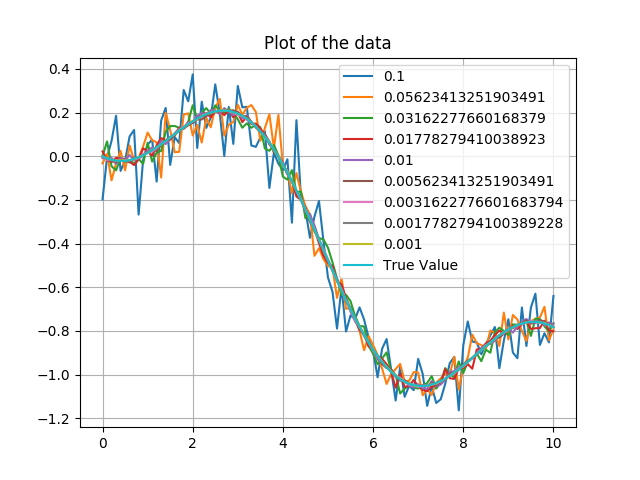
\includegraphics[scale=0.5]{Assignment_3_Qn3.png}
   	\caption{Time vs Value, for various error amounts}
   	\label{fig:allgraphs}
   \end{figure} 

 \subsection{Part 4}
 We have already defined the function, so we plot it now.
 \begin{minted}{python3}
figure(0)
plot(time,true_fn)
xlabel(r"$t$",size =20)
ylabel(r"true value",size =20)
grid(True)
\end{minted}
\begin{figure}[!tbh]
   	\centering
   	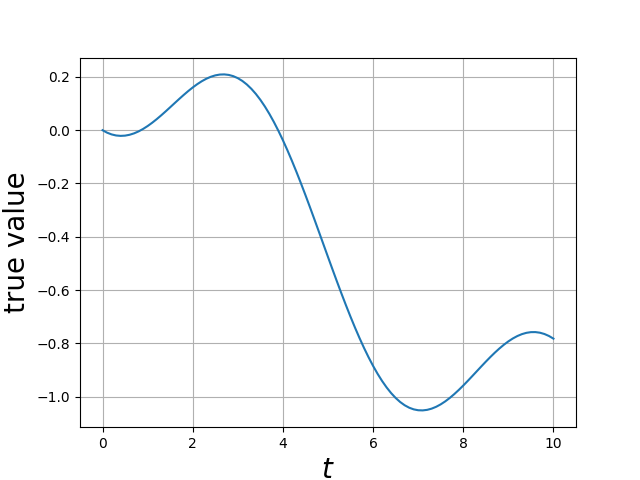
\includegraphics[scale=0.5]{Assignment_3_Qn4.png}
   	\caption{Plot the function (Without Matrix Multiplication)}
   	\label{fig:trueNoMatrix}
   \end{figure}
   
  
 \subsection{Part 5}
 We now generate a plot of the data with error bars.
 \begin{minted}{python3}
figure(1)
plot(time,c_[values[:,0],true_fn])
std = std(values[:,0]-true_fn)
errorbar(time[::5],values[:,0][::5],std,fmt='ro')
show()
\end{minted}

\begin{figure}[!tbh]
   	\centering
   	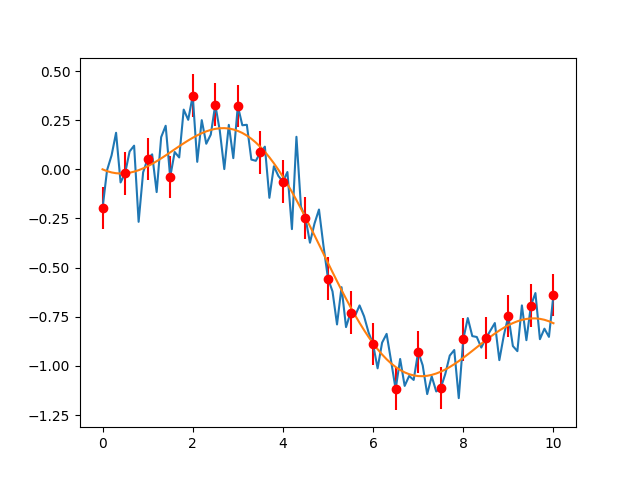
\includegraphics[scale=0.5]{Assignment_3_Qn5_Modified.png}
   	\caption{Function with Error Bars}
   	\label{fig:errorbars}
   \end{figure}

  
 \subsection{Part 6}
 We can also calculate the function using a matrix multiplication.
 \begin{minted}{python3}
 
def g_matrix(t,A=1.05,B=-0.105):
	J_val = sp.jn(2,t)
	t_val = t
	M = c_[J_val,t_val]
	x = array([A,B])
	return(matmul(M,x),M)


figure(0)
supposed_true = g_matrix(time)[0]
plot(time,supposed_true)
title("Plot using Matrix Multiplication")
xlabel(r"$t$",size =20)
ylabel(r"true value",size =20)
legend(["True Value"])
show()
\end{minted}

\begin{figure}[!tbh]
   	\centering
   	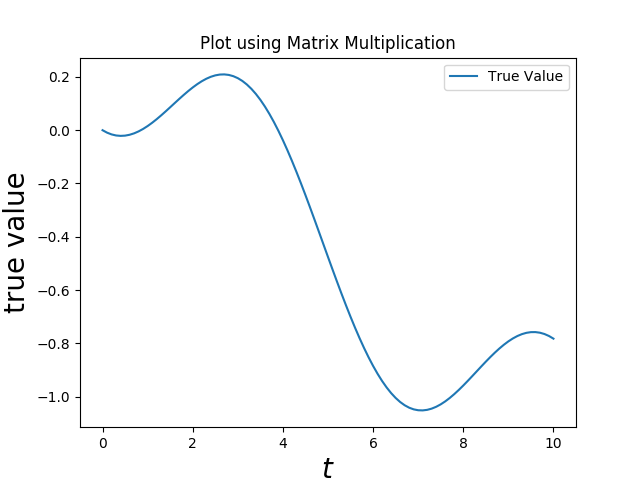
\includegraphics[scale=0.5]{Assignment_3_Qn6.png}
   	\caption{Using Matrix Multiplication to evaluate the function}
   	\label{fig:trueMatrix}
   \end{figure}

 \subsection{Part 7, 8}
 We can plot the mean square error for various values of A and B as a contour plot.
 \begin{minted}{python3}

def mse(data,assumed_model):
    return(sum(square(data-assumed_model))/101)


A_range = arange(0,2.1,0.1)
B_range = arange(-0.2,0.01,0.01)
figure(1)
e_matrix = zeros((len(A_range),len(B_range)))
for A in enumerate(A_range):
	for B in enumerate(B_range):
		e_matrix[A[0]][B[0]] = mse(values[:,0],g_matrix(time,A[1],B[1])[0])
contour_obj = contour(A_range,B_range,e_matrix,arange(0,20*0.025,0.025))
clabel(contour_obj,contour_obj.levels[0:5])
title("Contour Plot")
plot(1.05, -0.105,'ro', label = 'Exact Value')
annotate(s ="Exact Value",xy = [0.8,-0.100])
show()
\end{minted}

\begin{figure}[!tbh]
   	\centering
   	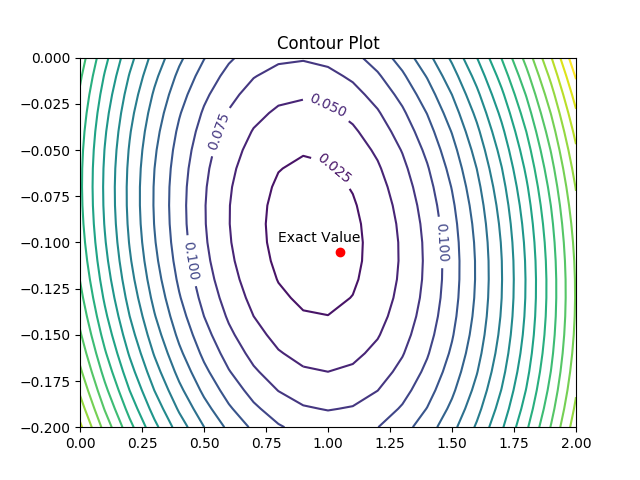
\includegraphics[scale=0.5]{Assignment_3_Qn8.png}
   	\caption{Contour Plot of MSE}
   	\label{fig:sample}
   \end{figure}


 \subsection{Part 9,10}
 We can calculate best estimate of A and B using linear least squares fitting.
 We plot the mean square error of the model in the estimated model vs actual model as a blue line.
 We plot the difference in A (expected vs actual) as red circles.
 We plot the difference in B (expected vs actual) as green circles.
 The error (blue line) grows exponentially versus Noise.
 \begin{minted}{python3}
l_mse_A = zeros((9))
l_mse_B = zeros((9))
l_mse_error = zeros((9))
for i in range(9):
	temp = linalg.lstsq(g_matrix(time)[1],values[:,i],rcond=None)
	l_mse_error[i] = temp[1][0]
	l_mse_A[i],l_mse_B[i] = temp[0]
figure(2)
plot(scl,l_mse_error)
plot(scl,absolute(l_mse_A-1.05),'ro')
plot(scl,absolute(l_mse_B+0.105),'go')
title("Error vs Noise")
show()
\end{minted}

\begin{figure}[!tbh]
   	\centering
   	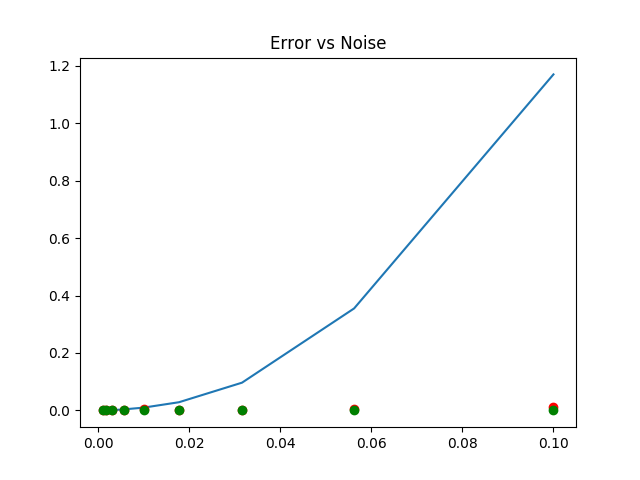
\includegraphics[scale=0.5]{Assignment_3_Qn10.png}
   	\caption{Error vs Noise}
   	\label{fig:EVN}
   \end{figure}


 \subsection{Part 11}
 We now replot the above using log log scales.
 The blue line shows that the error is linear on the log log scale
 \begin{minted}{python3}
figure(3)
loglog(scl,l_mse_error)
loglog(scl,absolute(l_mse_A-1.05),'ro')
loglog(scl,absolute(l_mse_B+0.105),'go')
title("Log Error vs Log Noise")
show()
\end{minted}
\begin{figure}[!tbh]
   	\centering
   	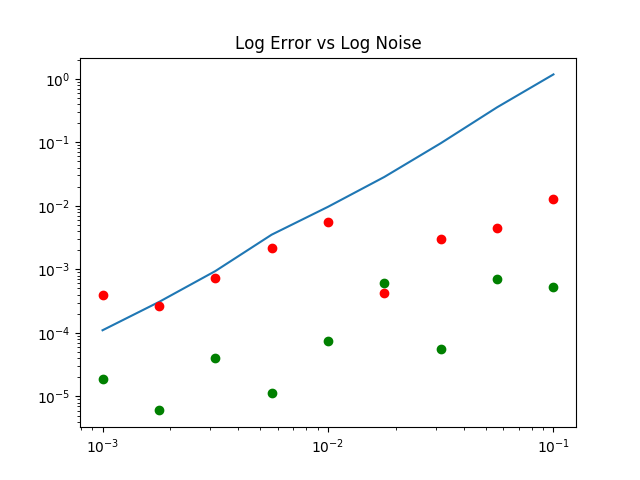
\includegraphics[scale=0.5]{Assignment_3_Qn11.png}
   	\caption{Log Error vs Log Noise}
   	\label{fig:loglog}
   \end{figure}

\section{Conclusions}
\begin{itemize}
    \item $\log(error)$ is linear with $\log(noise)$.
    \item Least Squares Fitting can be used to find a best fit for an overdetermined system of equations.
\end{itemize}
\end{document}



 